\section{Imitierendes Lernen}

Für Algorithmen des maschinellen Lernens wie z. B. RL, erweist die Skalierung zu höherdimensionalen Handlungsräumen ein großes Optimierungsproblem auf. \footcite[Vgl.][S. 3]{Hussein.2017}
Hinzu kommen Schwächen in der Anwendung von verstärkendem Lernen wie Handlungsstrategien in unerfahrenen Umgebungszuständen. \footcite[Vgl.][S. 1]{attia.2018}
Imitierendes Lernen (IL) kann hier als ein Vorschritt zur Optimierung von RL Modellen dienen, womit signifikante Belohnungsverbesserungen erzielt werden können. \footcite[Vgl.][S. 4]{Hussein.2017}
Ein Anwendungsgebiet des imitierenden Lernens ist die Robotik, in welchem ein chirurgischer Roboter durch Teleoperation bereits erfolgreich chirurgische Eingriffe demonstrieren konnte. \footcite[Vgl.][]{gao.2014}
Allgemeiner wird IL häufig eingesetzt, um menschliches Verhalten nachzuahmen und zu deren Aktionen zu beschleunigen. \footcite[Vgl.][S. 1]{attia.2018}
Das Ziel von IL ist hierbei eine Zuordnung zu erlernen zwischen den Beobachtungen und Aktionen von Expertendemonstrationen. \footcite[Vgl.][S. 1]{Hussein.2017}
Dadurch soll ein Roboter das ihm demonstrierte Verhalten reproduzieren und auch für unbekannte Szenarien generalisieren können. \footcite[Vgl.][S. 365]{fang.2019}
Problemstellungen können somit auf das Demonstrieren und Anlernen der Fähigkeit beschränkt werden, ohne dass explizite Anweisungen oder Belohnungsfunktionen programmiert werden müssen. \footcite[Vgl.][S. 1]{Hussein.2017}
IL stellt dabei einen passiven Ansatz dar, die Zielstrategie durch Beobachten der vollständigen Ausführungsabläufe zu erlernen. \footcite[Vgl.][S. 2]{attia.2018}
Dabei wird eine Ersatz-Verlustfunktion optimiert, welche die Diskrepanz zwischen der gewählten Aktion der parametrisierten Strategie $\pi_{\theta}$ und der des Experten $\psi$ misst. \footcite[Vgl.][S. 2f.]{Ashwin.2020}

Der typische Einsatzprozess von IL beinhaltet das Akquirieren von Demonstrationsbeispielen, deren Kodierung als Zustands-Aktions Paare und das Optimieren einer Strategie. \footcite[Vgl.][S. 3]{Hussein.2017}
Einzelne Prozessschritte können sich dabei je nach Anwendungsgebiet unterscheiden oder Nachfolgeprozesse, wie die Feinabstimmung mittels RL enthalten, was an Abbildung 3 deutlich wird.
\begin{figure}[htb]
    \centering
    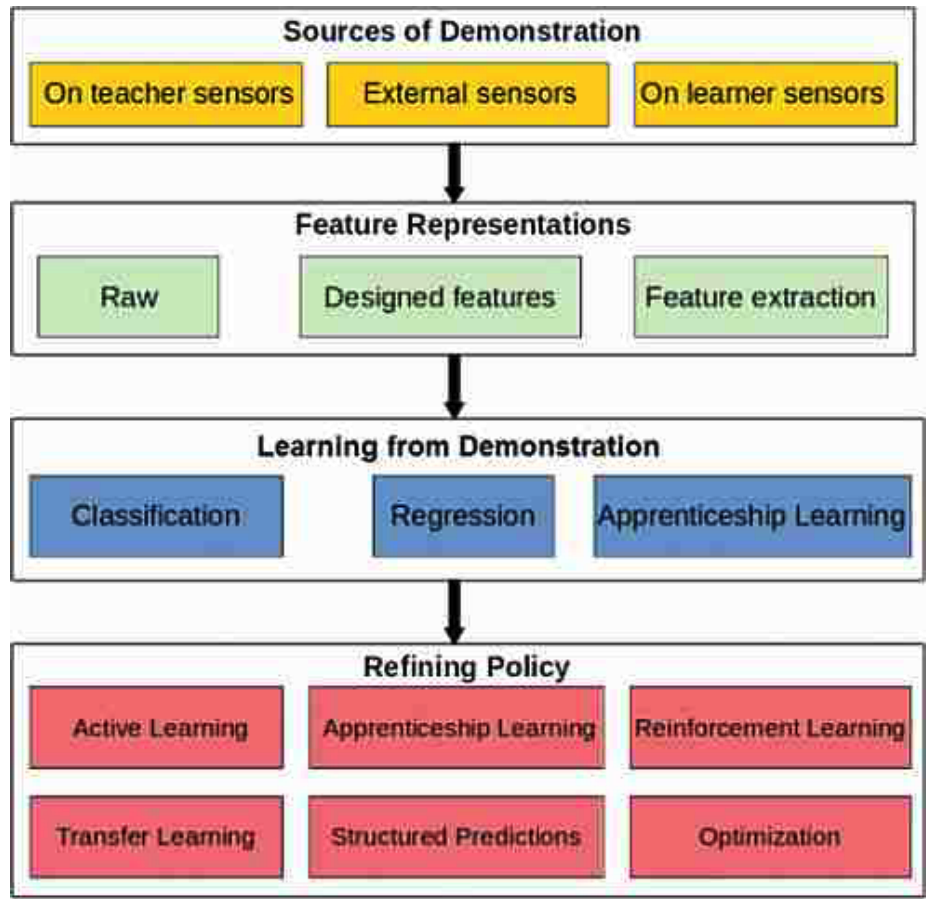
\includegraphics[height=7.2cm]{lib/graphics/IL flowchart.png}
    \caption[Ablaufdiagramm des imitierenden Lernens]{Ablaufdiagramm des imitierenden Lernens\footnotemark}
    \label{abb:IL-process-flowchart}
\end{figure}
\footnotetext{Enthalten in: \cite[][S. 4]{Hussein.2017}}

Algorithmen des imitierenden Lernens unterscheiden sich in der Literatur nach den Begriffen \textit{on-policy} und \textit{off-policy}. \footcite[Vgl.][S. 3]{Ashwin.2020}
Dabei werden zum einen erlernte Strategien in der Umgebung ausgeführt und mittels Experten evaluiert, zum anderen werden lediglich die Expertendemonstrationen verwendet. \footcite[Vgl.][S. 3]{Ashwin.2020}
DAgger stellt ein \textit{on-policy} Algorithmus dar, welcher zu jeder Iteration die Optimierung aller bisher beobachteten Zustands-Aktions Paare vornimmt. \footcite[Vgl.][S. 5]{attia.2018}
Behavioral Cloning als \textit{off-policy} Algorithmus erlernt hingegen die direkte Übersetzung der Zustands- und Umgebungsinformationen zu ihren Aktionen, ähnlich einem Label unter überwachtem Lernen. \footcite[Vgl.][S. 4]{fang.2019}

Insgesamt kann der Einsatz von IL unter anderem folgende Vorteile verzeichnen: \footcite[Vgl.][S. 1]{fang.2019}
\begin{itemize}
    \item Verbesserung der Anpassungsfähigkeit hinsichtlich neuer Umgebungen
    \item Erhöhung der Lerneffizienz aufgrund schnellerer Übertragung von Wissen
    \item Kompatibilität mit anderen Algorithmen des maschinellen Lernens wie z. B. RL
\end{itemize}

Aufgrund der interdisziplinären Natur von IL ergeben sich jedoch wie folgt auch eine Reihe von Herausforderungen: \footcite[Vgl.][S. 4f.]{Hussein.2017}
\begin{itemize}
    \item Der IL Prozess ist sowohl während der Sammlung von Demonstrationsdaten sowie während des Trainingsverlaufs anfällig für Rauschen und Fehler der Sensorik.
    \item Fähigkeiten, Aufbau und Freiheitsgrade des lernenden Modells und des Experten müssen bestmöglich übereinstimmen.
    \item Anwendungen lassen sich aufgrund ihres Echtzeitbezugs und Limitierungen der Rechenkapazitäten nur schwierig, hinsichtlich hoher Freiheitsgrade skalieren.
\end{itemize}